%\documentclass[12pt,letterpaper,final]{article}
\documentclass{acm_proc_article-sp}
\usepackage{url}
%\usepackage[dvips]{graphicx} 
%\usepackage{fullpage}
\begin{document}
%\oddsidemargin 0.25in 
%\textwidth 6.0in 
\title{Milestone 2: Literature Review and Design}

\numberofauthors{1}

\author{
\alignauthor 
Eliza Brock \\
       \affaddr{Rose-Hulman Institute of Technology}\\
       %\affaddr{1932 Wallamaloo Lane}\\
       %\affaddr{Wallamaloo, New Zealand}\\
       \email{brocker@rose-hulman.edu}
}
%\author{Eliza Brock}
%\date{\today}
\maketitle
%\tableofcontents
%\newpage

%Run spell check!


\section{Analysis of the Field}
\subsection{XML Processing}
The mainstream approaches to parsing and accessing XML data are DOM (Document Object Model) and SAX(Simple API for XML). DOM is a full featured in-memory representation of an XML document.  DOM can be very cumbersome when working with large documents and even the best of the widely-used DOM parsers has trouble with large documents. SAX  uses linear scanning to trigger SAX events as various datum are encountered.

The most interesting non-mainstream (or at least not mainstream to consumers of XML processing) of the data structures that can be used to index and store XML data for further processing are tree-to-table mapping, prefiltering, external-memory index structures and range labeling.  

Prefiltering frameworks\cite{huang:prefiltering} can make processing large XML files more feasible by returning slices of a large XML document to a client that can then use a SAX or DOM parser to complete the query.  

Range labeling is extremely convenient for processing containment queries\cite{chen:indexing}.





\subsection{XPath Processing}\cite{xpathspec}


The majority of the papers that I read on XPath and XPath processing focused on a specialized subset of XPath referred to as  ``navigational XPath'' or ``core XPath'' rather than the full XPath specification.   


%Complexity is described in: \cite{gottlob:complexity} and reading that paper more thorughly may be helpful if algorithm runtime becomes an issue for the final product.

One of the most useful things I picked up was some differentiation on the various properties of XPath fragments, from Bendikt's  ``Structural Properties of XPath fragments''\cite{benedikt:structural} which differentiates between downward vs. upward, recursive vs. nonrecursive, and qualifiedvs. non-qualified XPath fragments.

The two main optimizations that I have seen for XPath processing are query rewriting\cite{koch:processing} and the advent of streaming algorithms\cite{barton:streaming}.

Query rewriting focuses on preventing unnecessary document traversal by eliminating unnecessary steps.  Perhaps the most interesting of the algorithms for query rewriting is the Xaos algorithm\cite{barton:streaming} due to its incorporation of backward-axes.  There are several other algorithms that incorporate optimizations for only forward axes (e.g. XFilter, YFilter, XTrie, and TurboXPath).

Streaming algorithms work by processing the XPath expression as the document is scanned, thus bypassing the common requirement that an entire document by in memory before an expression can be evaluated.

\subsubsection{XPath Satisfiability with Schemas}
After reading about XPath satisfiability, I've come to the conclusion that it isn't a particularly interesting tangent to take for a pedagogical tool of this nature.

The basic approaches to satisfiability that I've read about thus far either  transform queries and trees into specialized calculi \cite{geneve:static}, incorporate the use DTDs\cite{benedikt:satisfiability}, or   focus on XML Schemas\cite{groppe:filtering}.

The calculus approach has an interesting application to pedagogical tools, in that it can be used to ``generate XML tree examples when the containment does not hold''\cite{geneve:static}, thus providing students with examples of \emph{why} their query does not or may not returns any results.

\section{Preliminary Research Results}

\subsection{Implementation Languages/Techniques}
\subsubsection{Implementation Language}
I will be using Haskell to implement this research project.  Haskell is a purely functional programming language that has good support for pattern matching and appears to have a large number of  libraries available that are applicable to the project at hand.
\subsubsection{Server/Web Framework}
For this project, I need a server with support for the following usage: automatic recompilation upon source change, session state, and the AJAX paradigm.  I considered the following approaches before finally settling on using HAppS\cite{HAppS}.  If HAppS does not work out, I will try the other options available in the order below:
	\begin{description}
	\item[HAppS] ``Haskell Application Server'' Features auto recompilation, optional state storage, and is designed for the "pattern of developing static web pages and using AJAX to populate them with dynamic content" \cite{HAppS}
	\item[WASH] ``Web Authoring System Haskell'' Supports for session persistence, and has been used in a number of production web services, good support for database access.\cite{WASH}
	\item[CGI libraries] Simplest approach.  However, using the CGI libraries directly would involve putting effort into work that isn't directly related to the project's end goals.
	\item[Others] HWS, SHWF, and other lesser known web frameworks written for Haskell.
\end{description}
	
\subsubsection{Javascript} 
 I'm looking into javascript libraries in order to facilitate the usage of XMLHttpRequest and dynamic content generation.  At this point I'm either going to use jQuery\cite{jquery} or write all the necesary javascript by hand.

I'll be using a technique similar to the one used in the script section of the 4umi javascript code samples\cite{4umi} to do some subquery-related highlighting.

\subsubsection{HTML}
I found several GPL'd HTML/javascript based org charts that look like they'll really fit the bill for displaying tree-based data.  I plan on using one of R.P. Bouman's Org Chart scripts to generate much of my in-browser XML view \cite{org02, org03}.  For my existing prototype, I am using version 3
of Bouman's scripts.

\subsection{Data Collection}
I have collected a number of XML files from various internet sources\cite{xml1,xml2,xml3} to use while testing the project.  However, few of them are properly licensed for the task at hand.  Since my needs for small easy-to-understand yet somewhat complex XML documents, I will probably end up writing my own sample documents later, rather than trying to find appropriate publicly licensed samples.




%%%%%%%%%%%%%%%%%%%%%%%%%%%%%%%%%%
\subsection{Algorithms Under Consideration}

\subsubsection{XML}
I'm particularly interested in creating a \emph{light-weight} DOM-esque framework in conjunction with a tree-to-table mapping and range labeling.

DOM will cover direct ancestor and descendant relationships, while tree-to-table mapping with range labeling will coordinate descendant-or-self axis and some of the other more complicated axes.

The enhanced indexing in \cite{chen:indexing} and the well specified axis relationships defined therein are extremely interesting.  I plan on investigating them more thoroughly, and, depending on my implementation I might choose to use Chen's indexing technique (modified to work in-memory rather than on-disk)  in lieu of my original plan of using a tree-to-table mapping with range labeling.

\subsubsection{XPath}
The W3C has an excellent reference for parsing XPath expressions, "Building a Tokenizer for XPath of XQuery" \cite{xpathtokenizer}, which will serve as an excellent guide for parsing strategies and writing a tokenizer for the XPath expressions.

I think that, based on the strategy I plan to take with partial parsing and monadic processing, that it may be possible to have a sort of pause-return-continue loop within the processing of XPath expressions, such that, at the end of each evaluation of a subexpression, the parser pauses to return the set of nodes that have been selected, and then waits for the input of an additional subexpression- at which point it will continue parsing from the point at which it left off, without repeating any unnecessary effort. 

Streaming algorithms \cite{barton:streaming} sound really interesting.  However, given the slightly-stateful, mostly-synchronous nature of the project's XPath processing I'm not sure that streaming algorithms work in this context.  

I'm certain that the streaming algorithms that work with backward axes wouldn't work with the "sub-expression at a time" approach that I plan on taking.  However, it would be very interesting to use forward-axis only streaming processing. 

The concept of streaming processing might be better saved for future work on the project; perhaps with the inclusion of a feature in which the user can manually specify very large documents.  Given the current restrictions I have in place for the sake of in-browser usability, the gains from streaming parsing would be negligible.


%%%%%%%%%%%%%%%%%%%%%%%%%%%%%%%%%%%%%%%%%%%


\subsection{Updated Timeline}
\begin{figure}[!htpb]
\centering
\psfig{file=process.ps, width=3in, height=2.5in,}
%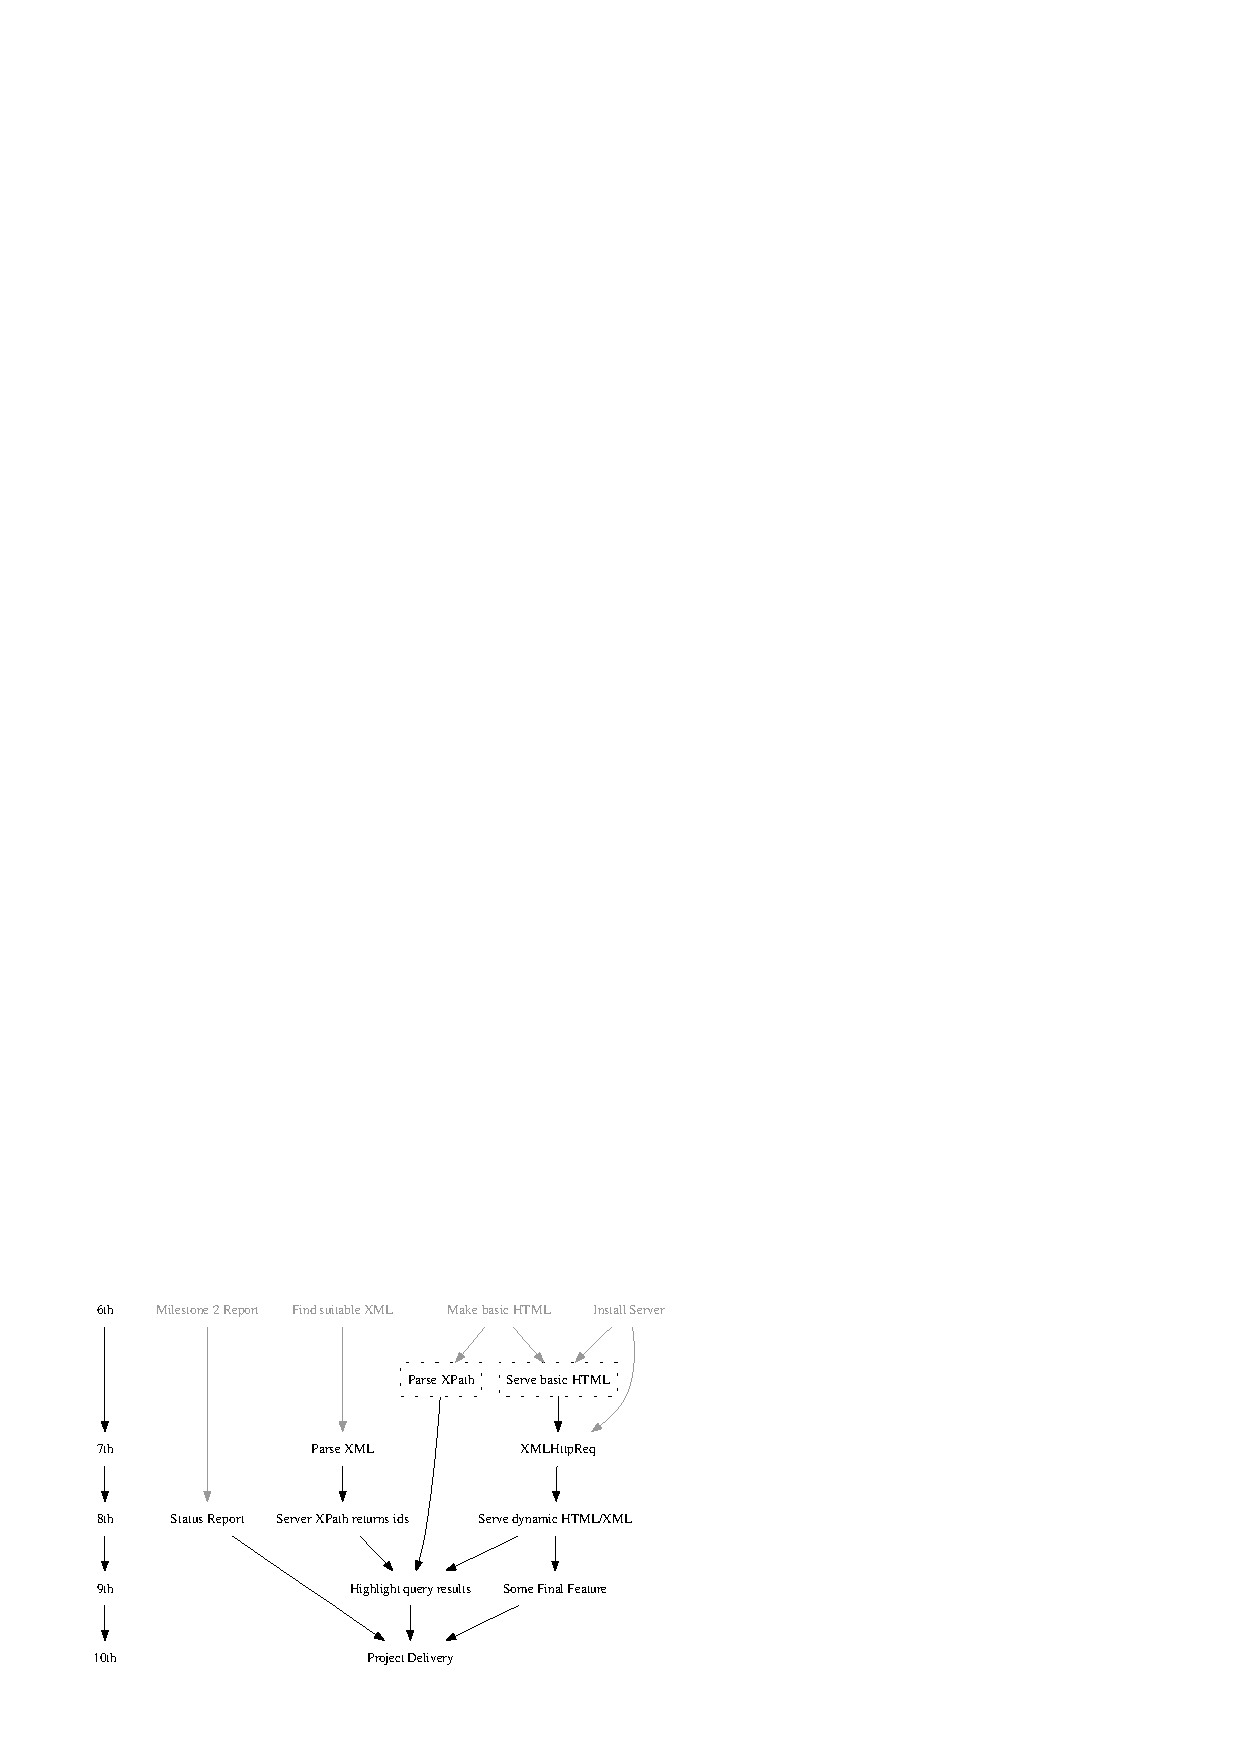
\includegraphics[width=\textwidth]{process}
\caption{Schedule (Grey is completed, Dotted is in progress)}
\end{figure}

%\cite{chen:indexing} was very useful and should be re-read.
%\newpage
\newpage
\nocite{gottlob:complexity}
\nocite{marx:semantic}
\nocite{xmlspec}
\bibliographystyle{abbrv}
\bibliography{uno}

\end{document}